\section{Main result: signal withdrawal exposes a commitment difference}
\label{sec:death-results}

\subsection{Baseline agreement and its exact scope}

Complete reachable-state enumeration yields \DRBasePlusStates{} states and
\DRBaseMinusStates{} states for the two sustained-stimulation quotients.
Each has exactly three reachable singleton terminal components: survival,
apoptosis and necrosis. This is exact agreement of terminal-fate predictions,
not an assertion about matching probabilities or every transient trajectory.
An expanded exact subset-product search found a 12-action word admitted by
DR-FB+ but not DR-FB-, without changing the models or interface:
\[
\begin{split}
w={}&\mathrm{MPT}\!\uparrow,\ \mathrm{CASP3}\!\uparrow,\
\mathrm{CASP3}\!\downarrow,\ \mathrm{NFkB}\!\uparrow,\\
&\mathrm{NFkB}\!\downarrow,\ \mathrm{MPT}\!\downarrow,\
(\mathrm{CASP3}\!\uparrow,\ \mathrm{CASP3}\!\downarrow)^3 .
\end{split}
\]
The superscript denotes three repetitions of the action pair, not physical
time. Exact propagation, an independent sparse reachability calculation and
mCRL2 confirm acceptance only in DR-FB+. A reconstructed 53-update accepting
path also satisfies the original full 28-node rules. Therefore global
sustained trace equality is refuted, DR-FB- cannot weakly simulate DR-FB+,
and the two systems are not weakly bisimilar. The reverse inclusion remains unresolved;
its unknown status does not prevent the inequality decision. This is a
qualitative model counterexample, not a measured oscillatory trajectory.

The more specific comparison at the shared state identified below is fully
resolved. With TNF kept on, each continuation has \DRLocalBaseStates{} states
and \DRLocalBaseEdges{} silent edges, and no further observable action.
Both are strongly and weakly bisimilar and have exact weak language
$\{\epsilon\}$. The equality concerns continuations from that state, not
the complete systems from their original physiological initial condition.

\begin{figure}[t]
\centering
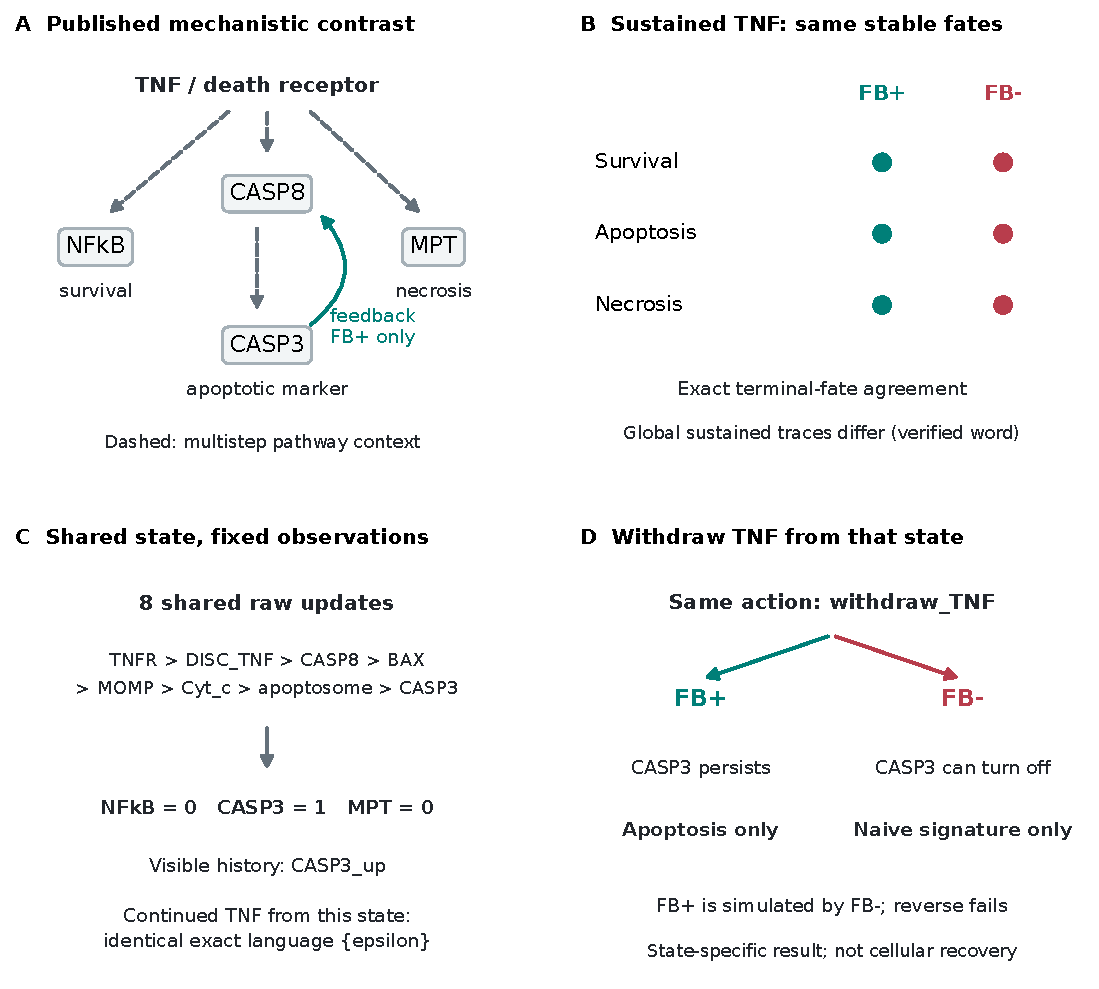
\includegraphics[width=\textwidth]{R3_Fig1.pdf}
\caption{Fixed-interface commitment comparison. (A) Mechanistic context, with
the literature-described CASP3-to-CASP8 feedback highlighted; dashed connectors
summarize multistep pathways, not direct molecular interactions.
(B) Both sustained-stimulation models reach the same three stable fates.
(C) An automatically extracted common history reaches the same retained
state; with continued TNF, both continuations have language $\{\epsilon\}$.
(D) Withdrawal from that state yields persistent CASP3 and an apoptotic
terminal fate for DR-FB+, but permits CASP3 loss and only the naive terminal
signature for DR-FB-. Counts and relations refer to exact retained-state
executions. No event count is converted to physical time.}
\label{fig:death-commitment}
\alttext{Four panels show the feedback hypothesis, matching baseline fates,
a shared CASP3-positive history, and different TNF-withdrawal continuations.}
\end{figure}

\subsection{A common history and a state-specific commitment witness}

The deterministic breadth-first search selects the first shared reachable state
satisfying persistent CASP3 and a unique apoptotic terminal future after
withdrawal in DR-FB+, versus a unique naive terminal future in DR-FB-.
One shortest raw-update path to this state is
\[
\begin{split}
&\mathrm{TNFR}\!\uparrow,\ \mathrm{DISC\_TNF}\!\uparrow,\
\mathrm{CASP8}\!\uparrow,\ \mathrm{BAX}\!\uparrow,\
\mathrm{MOMP}\!\uparrow,\\
&\mathrm{Cyt\_c}\!\uparrow,\ \mathrm{apoptosome}\!\uparrow,\
\mathrm{CASP3}\!\uparrow .
\end{split}
\]
All eight updates and the resulting retained vector are available in both
variants. The visible projection is $h=\texttt{CASP3\_up}$.
At this state, TNF, FADD, ATP, cIAP, TNFR, DISC\_TNF, CASP8, BAX, MOMP,
Cyt\_c, apoptosome and CASP3 are one; all other retained components are zero.
Thus the selected state is fully specified, not merely a pair of matching
marker values. The automatic selection is minimal in raw-event depth among
the states satisfying this criterion; it is not a claim of a globally shortest
biological observation or of a unique commitment state.

When withdrawal is permitted from this state, the continuations have
\DRLocalPlusStates{} states/\DRLocalPlusEdges{} edges and
\DRLocalMinusStates{} states/\DRLocalMinusEdges{} edges, respectively.
Write them $K_+$ and $K_-$. Exact checks give
\[
 K_+\weakpre K_-,\qquad K_-\not\weakpre K_+,\qquad
 K_+\not\weaksim K_-.
\]
The distinguishing trace in $K_-$ is
$\texttt{withdraw\_TNF}\,\texttt{CASP3\_down}$, absent from $K_+$.
The independent deletion-game certificate covers every defending weak reply,
not one conveniently chosen successor. Its dependency ranks decrease until
CASP3 deactivation has no matching action. Production predicates and mCRL2
agree on bisimulation and exact traces; both simulation directions are also
checked by the independent game.

The direction is important: $K_-$ can match the fewer observable actions of
$K_+$, but $K_+$ cannot match the additional deactivation response of $K_-$.
This is not a ranking of biological quality or survival. After immediate
withdrawal, $K_+$ retains CASP3 along every continuation and reaches only
apoptosis, whereas $K_-$ reaches only the model's naive signature. The latter
is a marker-level logical outcome, not evidence that an apoptotic cell can
return to viability.

\subsection{What the shared observation does and does not identify}

The visible history $h$ alone is compatible with \DRHistoryStates{} hidden
states in each sustained model. Aggregating complete post-withdrawal futures
over all such states gives
\[
\begin{split}
\mathrm{Futures}_+(h,\mathrm{withdraw})
 &=\{\mathrm{apoptosis},\mathrm{naive},\mathrm{necrosis}\},\\
\mathrm{Futures}_-(h,\mathrm{withdraw})
 &=\{\mathrm{naive},\mathrm{necrosis}\}.
\end{split}
\]
Therefore the difference is not confined to an arbitrarily paired pair of
hidden states. However, $h$ does not imply that every compatible DR-FB+ state
is irreversibly apoptotic. The full state witness and the history-aggregated
future sets answer different questions and are reported separately.

The complete withdrawal-aware systems have \DRControlPlusStates{} and
\DRControlMinusStates{} reachable states. Exact subset propagation gives a
DR-FB--only trace
$\texttt{CASP3\_up}\,\texttt{withdraw\_TNF}\,\texttt{CASP3\_down}$;
the defending DR-FB+ subset is empty after its last action. A trace in the
opposite direction is
$\texttt{withdraw\_TNF}\,\texttt{CASP3\_up}\,\texttt{CASP3\_down}\,
\texttt{CASP3\_up}$.
These exact counterexamples refute both global trace inclusions and hence both
global weak-simulation directions; they require no exhaustive language
enumeration. Ordinary trace comparison can detect differences under both the
sustained and withdrawal protocols. We do not present this biological
case as the stronger equal-global-trace/different-branching phenomenon of
Example~\ref{ex:branching}.

The exhaustive scan considers every reachable history of exactly $k$ raw
updates before withdrawal, for $0\leq k\leq40$, with complete future
reachability thereafter. An apoptotic terminal future first becomes possible
in DR-FB+ after one hidden TNFR update; persistent-CASP3 commitment first appears
at $k=\DRDepth{}$, for \DRFirstCommitted{} of \DRDepthStates{} reachable
states at that depth. It never occurs in DR-FB- over this scan. State counts
are not path probabilities. No artificial stutters are added at terminal
states, no physical duration is assigned, and this first possible depth is
not a universal time at which all modeled cells commit.

\subsection{Prospective discriminator and evidential status}

The model-derived discriminator is a pulse/withdrawal comparison at a
CASP3-positive stage, followed by the joint observation of CASP3 persistence,
NFkB activity and MPT, with ATP status supporting fate classification.
Monitoring the other two markers matters: CASP3 loss accompanied by a change
in the necrotic branch is not the same trace as isolated CASP3 loss after
withdrawal. The three-marker history does not uniquely locate the hidden
witness state; more detailed state assessment would be needed to test its
state-specific claim. We specify no concentration, cell line, elapsed time or
selective experimental feedback inhibitor that these logical models cannot
justify. Ligand withdrawal and the feedback hypothesis originate in the
Calzone study.\cite{Calzone2010} Our added result is the explicit relational
and reachable-future account, not a newly proposed biological mechanism.

\begin{table}[t]
\tbl{Specified assumptions, computed results, and absent evidence in the
death-receptor comparison.\label{tab:evidence-status}}{
\small\setlength{\tabcolsep}{4pt}
\begin{tabular}{@{}>{\raggedright\arraybackslash}p{0.31\textwidth}>{\raggedright\arraybackslash}p{0.64\textwidth}@{}}
\toprule
Item & Evidential status\\
\colrule
CASP3-to-CASP8 feedback & Published model assumption; its removal was already studied.\\
Markers and withdrawal & Fixed interface and intervention declared before relation results.\\
Baseline terminal fates & Computed agreement: survival, apoptosis, necrosis.\\
Shared-state continuations & Exact sustained equality; one-way simulation and unequal traces with withdrawal.\\
Global sustained traces & Equality refuted by a verified 12-action word; reverse inclusion undecided.\\
Witness and fate persistence & Automatically computed; all defending replies checked.\\
Discriminating observation & Model-derived implication of a published perturbation.\\
Wet-lab confirmation & No new experimental validation; naive is not demonstrated cellular recovery.\\
\botrule
\end{tabular}}
\end{table}
